\documentclass[11pt]{article}

\usepackage[margin=1in]{geometry}
\usepackage[utf8]{inputenc}
\usepackage{xcolor}
\usepackage{tikz}
\usetikzlibrary{arrows.meta,positioning,fit,calc}

\title{Enterprise World Model: Revised Architecture}
\author{}
\date{}

\begin{document}

\maketitle

\section*{Overview}

Ok so this is the new architecture for my model that I’m thinking. It keeps a lot of the same verifier logic that worked well with the last version, but this one more explicitly encodes a more generalizable IR layer and a dynamics model, and also a way to extend easily to write-based tasks.

\section*{Symbolic IR}

The IR layer will still have the InstanceFrame and ExecutionState from the last iteration. The InstanceFrame gets generated by the base LLM at the beginning, encodes things like the goal, constraints, output contract. The ExecutionState, is basically a belief-state that tracks what evidence has been collected, what needs to be resolved, actions taken, which should help resolve failures where long interactions make the model start to hallucinate.

There will also be a new environment IR layer that encodes the info about the state of the environment, like object schema, entity relationships, and, for write-tasks, the extracted symbolic flows based on triggers and preconditions. I’ve done some thinking and I’ve determined that maybe the read-task equivalent of having learned workflow graphs for write-tasks (like in WoW) would be exposing a sort of affordance graph where the agent is exposed to what information can immediately be queried based on the current evidence collected. As opposed to centering around events and flows, this representation centers around objects and their relationships, which can guide these read-flows in a similar manner to how the symbolic layer would guide write-flows. I was also thinking about if there’s a way to mine data such that we could determine full read-based workflows conditioned on triggers, but I determined that read operations are not as causally related as writes are, so for now I’m going to stick with this information-reachability idea.

\section*{Action Selection}

As suggested by Sandeep, I’ll be using a Salesforce MCP server for execution instead of pure ReAct. Instead of having a precompiled action space like earlier, this model will be exposed to the Salesforce MCP server’s tools. Salesforce actually has separate MCP servers depending on the nature of the task. For this specific benchmark, we can expose the SObject-Reads server. I’ll also readjust the baseline numbers appropriately using this same MCP tooling.

\section*{Learned world model}

This is the next-state predictor part of the EWM, and for write operations, predicts the state diff based on the current state and the proposed action. This will be fine tuned with SFT over data mined pairs from the sandbox (state, action $\rightarrow$ next state).

\section*{Verifiers}

This uses the same logic as the loop from the previous version, including privacy checks to prevent confidential information from being disclosed and ensuring enough supported evidence was collected in the ExecutionState to return a final answer to the user.

\section*{Implementation progression}

Initially, to get this framework working on the current benchmark, the most important components are implementing this new generic intermediate representation and configuring the MCP tool call space. This completes a version of the EWM in which we have an intermediate representation, a symbolic layer guiding actions, and verifiers to check important actions. I don’t think having a full next-state predictor with a world model doesn’t make sense in this benchmark since read operations are cheap and not something to necessarily gate. This is why the next phase of implementation would then be mining the Salesforce sandbox (should be free) with augmented workflow templates to generate the flows needed to create a flow symbolic layer and fine tune our world model so that it is compatible with write operations, if we ever decide to test that. But I even think in this read-only benchmark, we have a corollary that is a natural extension of our full EWM framework.

\section*{Architecture Diagram}

\begin{figure}[h!]
\centering
\resizebox{0.95\textwidth}{!}{%
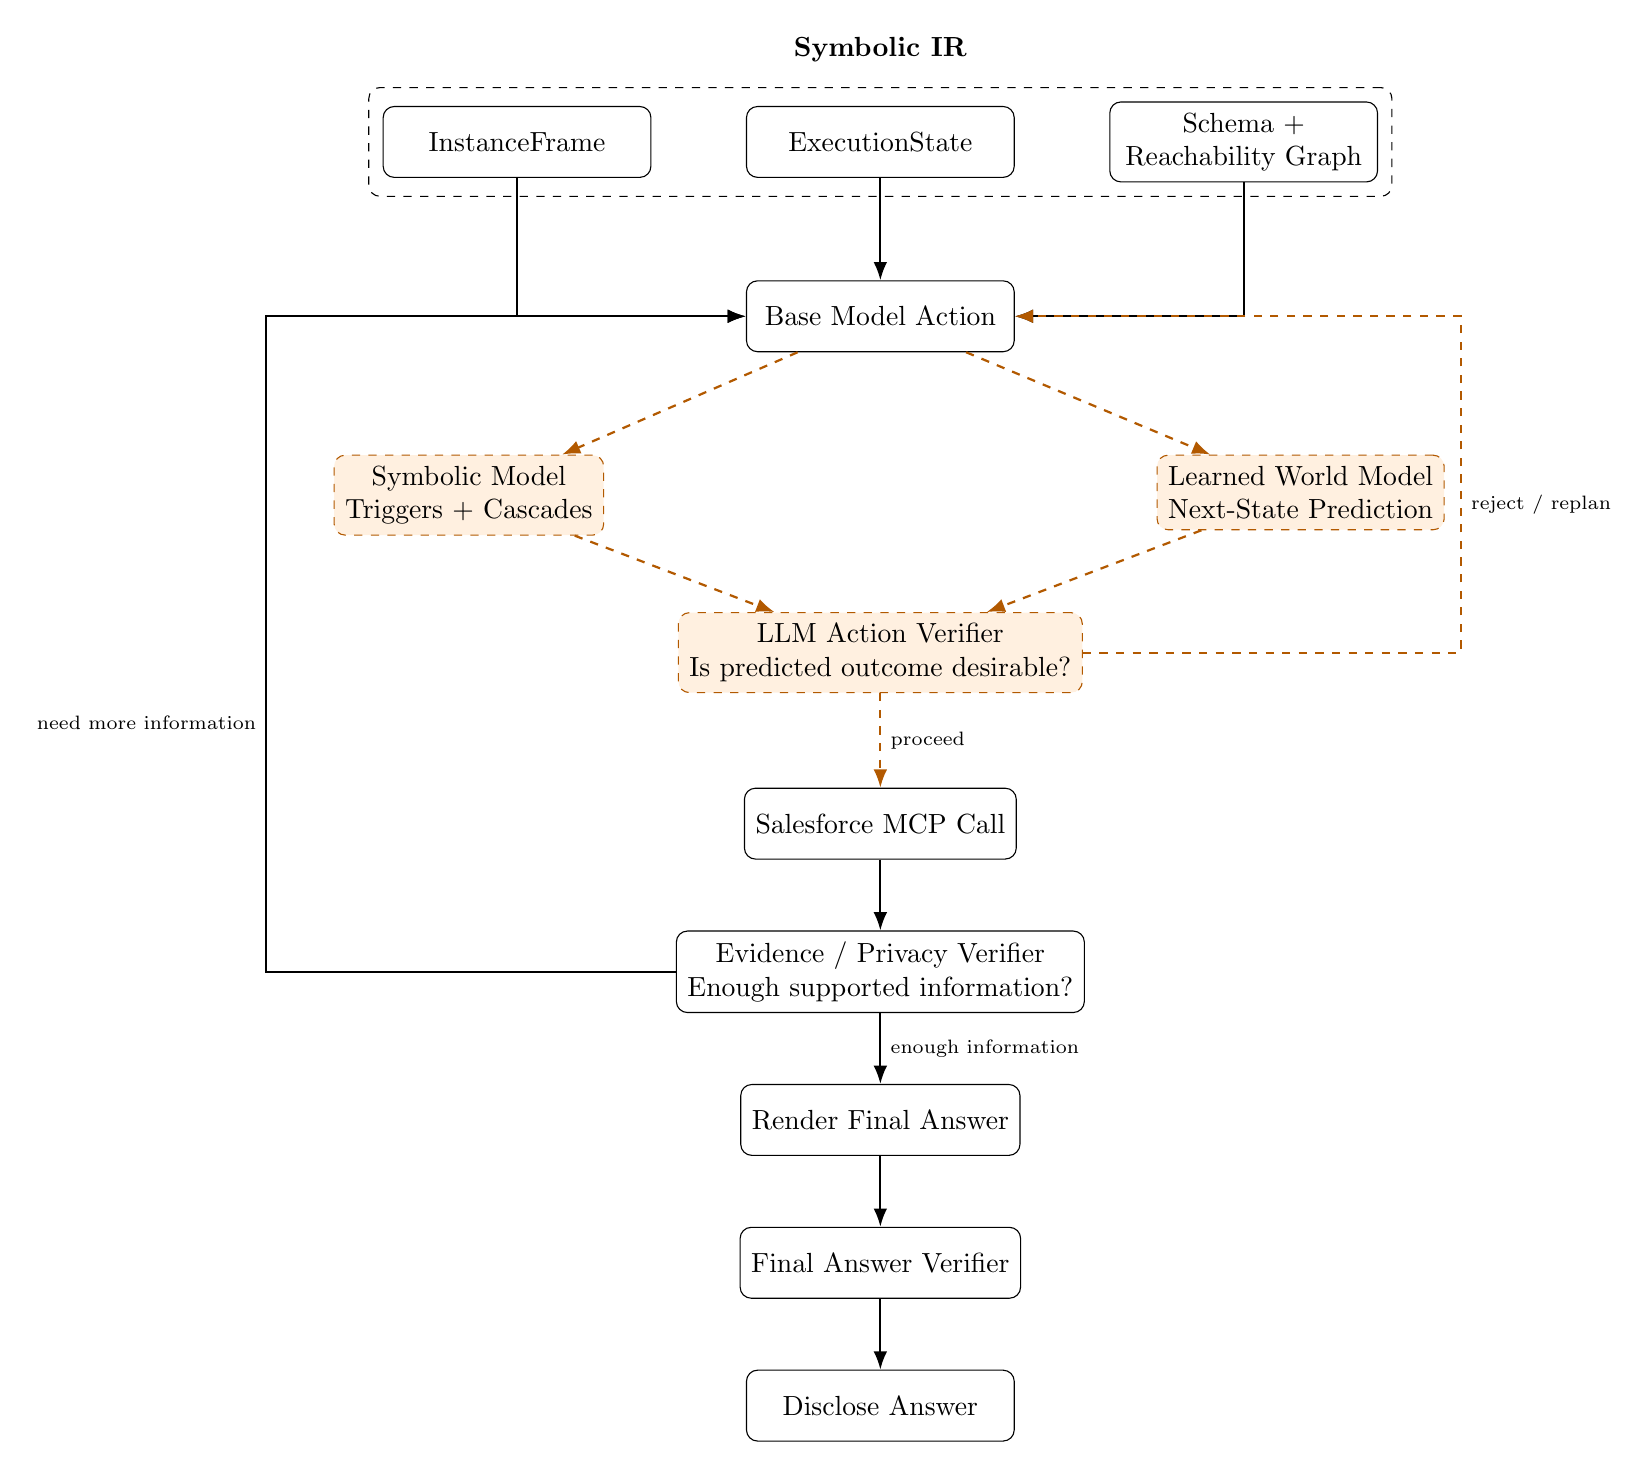
\begin{tikzpicture}[
    >=Latex,
    node distance=9mm and 12mm,
    box/.style={
        draw,
        rounded corners,
        align=center,
        minimum width=34mm,
        minimum height=9mm,
        inner sep=4pt
    },
    writebox/.style={
        draw=orange!70!black,
        fill=orange!12,
        dashed,
        rounded corners,
        align=center,
        minimum width=34mm,
        minimum height=9mm,
        inner sep=4pt
    },
    arrow/.style={->,thick},
    writearrow/.style={->,thick,dashed,draw=orange!70!black}
]

% Symbolic IR inputs
\node[box] (frame) {InstanceFrame};
\node[box, right=of frame] (state) {ExecutionState};
\node[box, right=of state] (env) {Schema +\\Reachability Graph};

\node[box, below=13mm of state] (model) {Base Model Action};

\draw[arrow] (frame) |- (model);
\draw[arrow] (state) -- (model);
\draw[arrow] (env) |- (model);

% Optional write-oriented prediction branch
\node[writebox, below left=13mm and 18mm of model] (sym)
{Symbolic Model\\Triggers + Cascades};

\node[writebox, below right=13mm and 18mm of model] (wm)
{Learned World Model\\Next-State Prediction};

\draw[writearrow] (model) -- (sym);
\draw[writearrow] (model) -- (wm);

\node[writebox, below=15mm of model, yshift=-18mm] (actionver)
{LLM Action Verifier\\Is predicted outcome desirable?};

% Straight parallel outputs into the action verifier
\draw[writearrow] (sym) -- (actionver);
\draw[writearrow] (wm) -- (actionver);

% Pre-execution rejection loop routed outside the right side
\draw[writearrow]
(actionver.east)
-- ++(48mm,0)
|- node[pos=0.22,right,align=center]
{\scriptsize reject / replan}
(model.east);

% MCP execution only after the prediction/verifier path
\node[box, below=12mm of actionver] (mcp) {Salesforce MCP Call};
\draw[writearrow] (actionver) -- node[right]{\scriptsize proceed} (mcp);

% Post-execution evidence/privacy check
\node[box, below=of mcp] (ver)
{Evidence / Privacy Verifier\\Enough supported information?};

\draw[arrow] (mcp) -- (ver);

% Need-more-information loop routed outside the left side so it avoids Symbolic Model
\draw[arrow]
(ver.west)
-- ++(-52mm,0)
|- node[pos=0.19,left,align=center]
{\scriptsize need more information}
(model.west);

% Final answer path
\node[box, below=of ver] (draft) {Render Final Answer};
\draw[arrow] (ver) -- node[right]{\scriptsize enough information} (draft);

\node[box, below=of draft] (finalver) {Final Answer Verifier};
\node[box, below=of finalver] (answer) {Disclose Answer};

\draw[arrow] (draft) -- (finalver);
\draw[arrow] (finalver) -- (answer);

% Only the actual symbolic IR inputs are grouped
\node[
    draw,
    dashed,
    rounded corners,
    fit=(frame)(state)(env),
    inner sep=5pt
] (irgroup) {};

\node[above=2mm of irgroup.north] {\textbf{Symbolic IR}};

\end{tikzpicture}%
}

\caption{Simplified EWM architecture. The dashed orange path represents the symbolic and learned prediction components used when pre-execution world modeling is needed.}

\end{figure}

\end{document}
